\documentclass{article}
\usepackage[a4paper,landscape,margin=0.5in]{geometry}
\usepackage{tikz}
\usetikzlibrary{graphs}
\pagestyle{empty}
\begin{document}
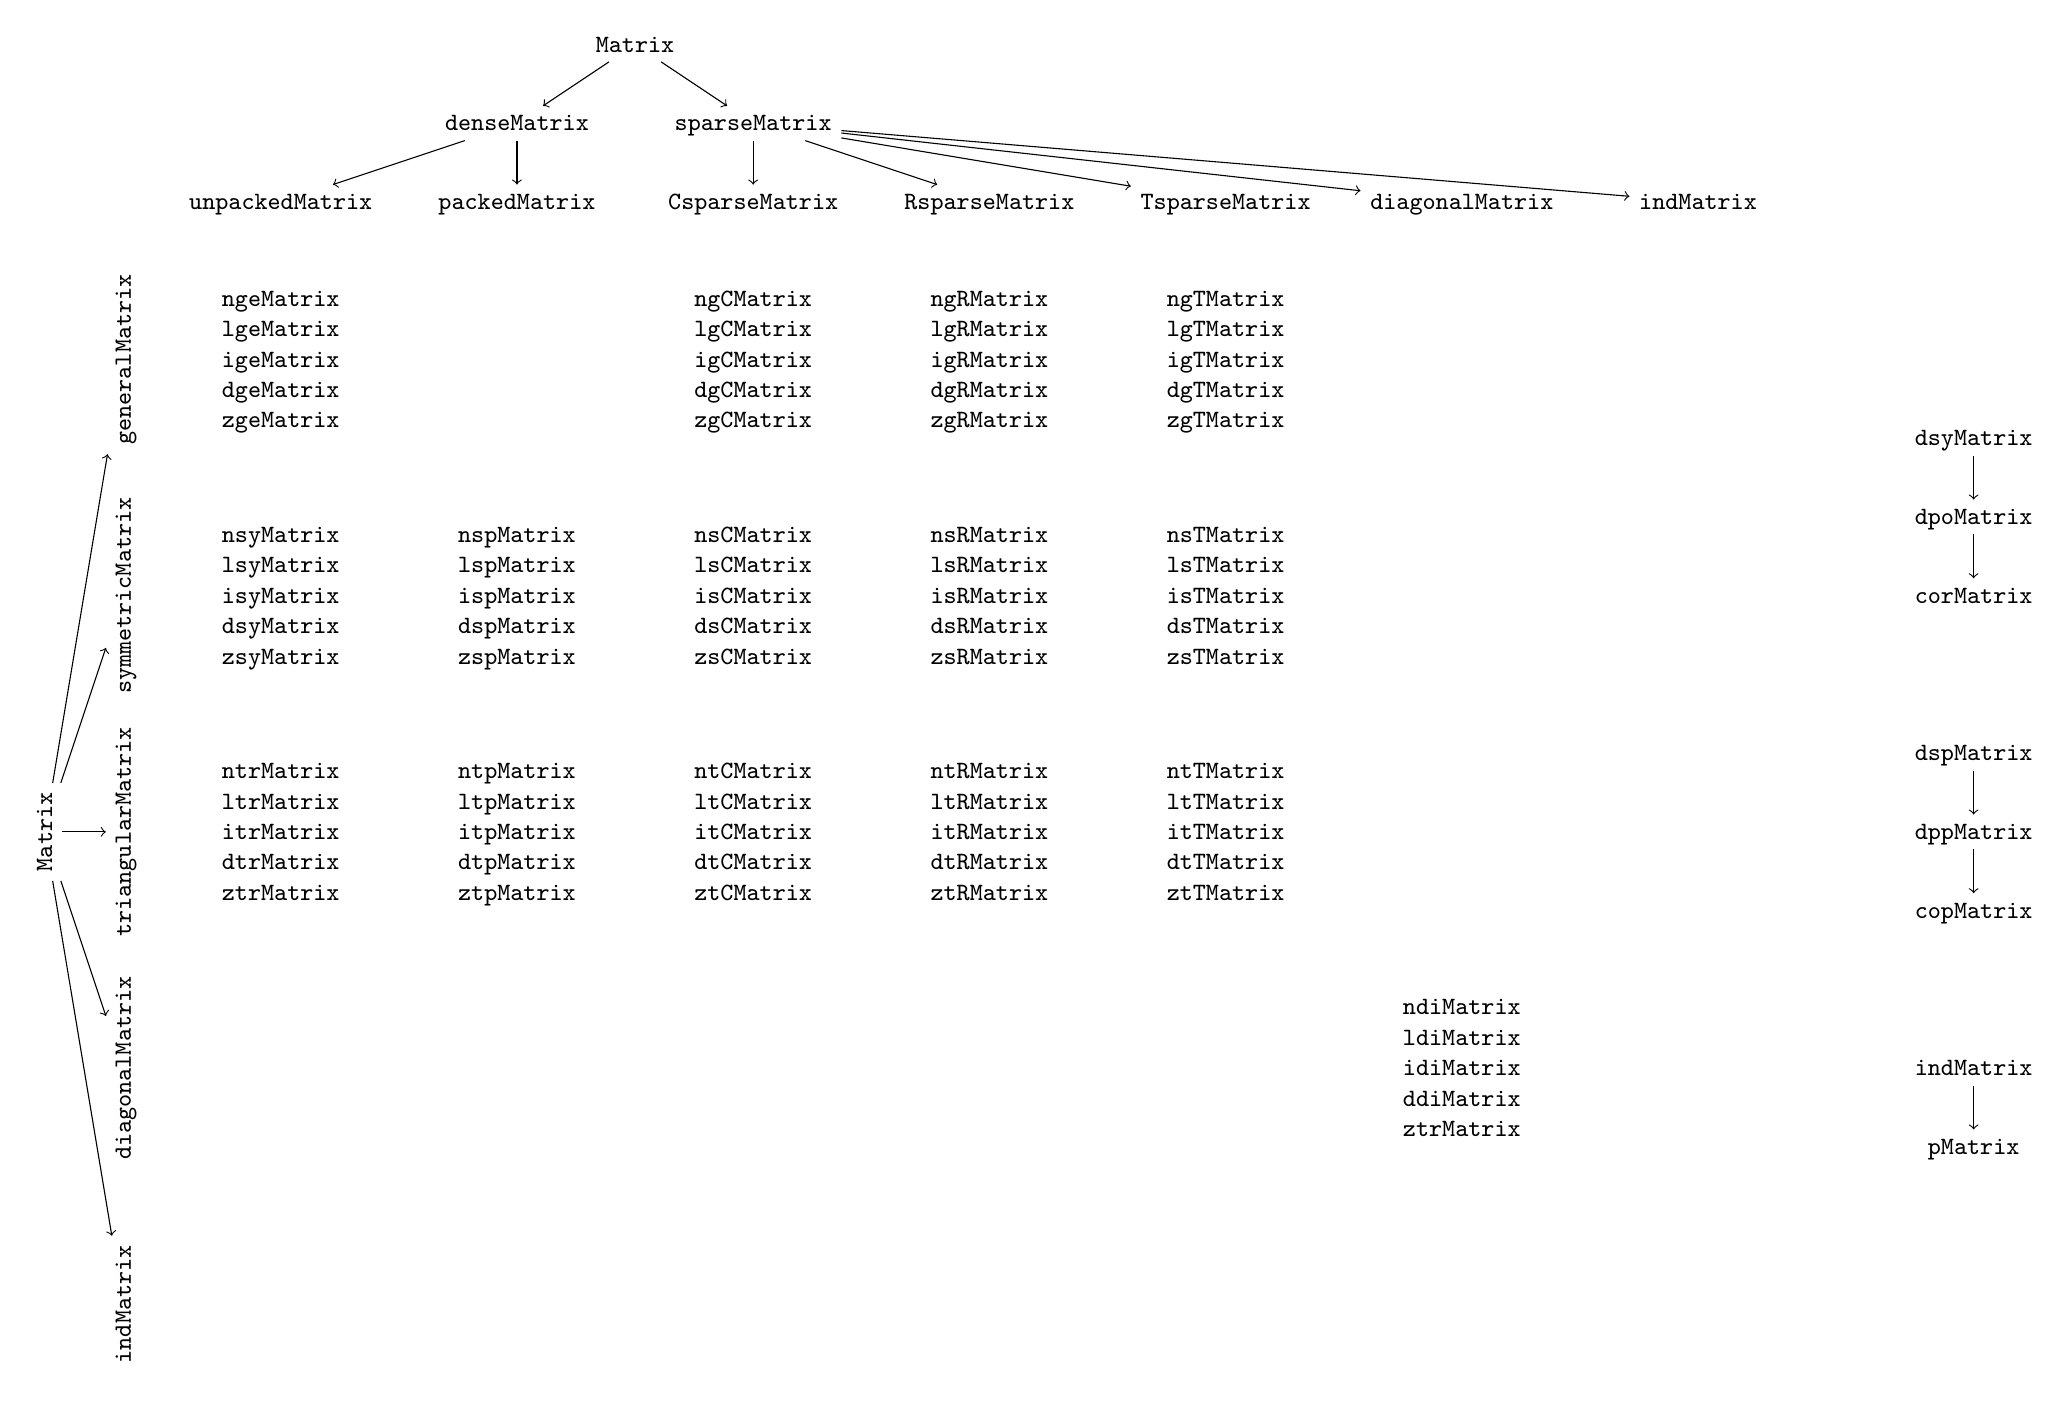
\begin{tikzpicture}[font=\small \tt,text depth=0pt,align=right]
\graph [no placement]
{
            Matrix1[x=- 7.5,y=-10,rotate=90,as=          Matrix],

     generalMatrix1[x=- 6.5,y=- 4,rotate=90,as=   generalMatrix],
   symmetricMatrix1[x=- 6.5,y=- 7,rotate=90,as= symmetricMatrix],
  triangularMatrix1[x=- 6.5,y=-10,rotate=90,as=triangularMatrix],
    diagonalMatrix1[x=- 6.5,y=-13,rotate=90,as=  diagonalMatrix],
         indMatrix1[x=- 6.5,y=-16,rotate=90,as=       indMatrix],

            Matrix2[x=  0.0,y=  0,rotate= 0,as=          Matrix],

       denseMatrix2[x=- 1.5,y=- 1,rotate= 0,as=     denseMatrix],
      sparseMatrix2[x=  1.5,y=- 1,rotate= 0,as=    sparseMatrix],

    unpackedMatrix2[x=- 4.5,y=- 2,rotate= 0,as=  unpackedMatrix],
      packedMatrix2[x=- 1.5,y=- 2,rotate= 0,as=    packedMatrix],

     CsparseMatrix2[x=  1.5,y=- 2,rotate= 0,as=   CsparseMatrix],
     RsparseMatrix2[x=  4.5,y=- 2,rotate= 0,as=   RsparseMatrix],
     TsparseMatrix2[x=  7.5,y=- 2,rotate= 0,as=   TsparseMatrix],
    diagonalMatrix2[x= 10.5,y=- 2,rotate= 0,as=  diagonalMatrix],
         indMatrix2[x= 13.5,y=- 2,rotate= 0,as=       indMatrix],

  Lge[x=- 4.5,y=- 4,as={ngeMatrix \\ lgeMatrix \\ igeMatrix \\ dgeMatrix \\ zgeMatrix}],
  Lgp[x=- 1.5,y=- 4,as={          \\           \\           \\           \\          }],
  LgC[x=  1.5,y=- 4,as={ngCMatrix \\ lgCMatrix \\ igCMatrix \\ dgCMatrix \\ zgCMatrix}],
  LgR[x=  4.5,y=- 4,as={ngRMatrix \\ lgRMatrix \\ igRMatrix \\ dgRMatrix \\ zgRMatrix}],
  LgT[x=  7.5,y=- 4,as={ngTMatrix \\ lgTMatrix \\ igTMatrix \\ dgTMatrix \\ zgTMatrix}],

  Lsy[x=- 4.5,y=- 7,as={nsyMatrix \\ lsyMatrix \\ isyMatrix \\ dsyMatrix \\ zsyMatrix}],
  Lsp[x=- 1.5,y=- 7,as={nspMatrix \\ lspMatrix \\ ispMatrix \\ dspMatrix \\ zspMatrix}],
  LsC[x=  1.5,y=- 7,as={nsCMatrix \\ lsCMatrix \\ isCMatrix \\ dsCMatrix \\ zsCMatrix}],
  LsR[x=  4.5,y=- 7,as={nsRMatrix \\ lsRMatrix \\ isRMatrix \\ dsRMatrix \\ zsRMatrix}],
  LsT[x=  7.5,y=- 7,as={nsTMatrix \\ lsTMatrix \\ isTMatrix \\ dsTMatrix \\ zsTMatrix}],

  Ltr[x=- 4.5,y=-10,as={ntrMatrix \\ ltrMatrix \\ itrMatrix \\ dtrMatrix \\ ztrMatrix}],
  Ltp[x=- 1.5,y=-10,as={ntpMatrix \\ ltpMatrix \\ itpMatrix \\ dtpMatrix \\ ztpMatrix}],
  LtC[x=  1.5,y=-10,as={ntCMatrix \\ ltCMatrix \\ itCMatrix \\ dtCMatrix \\ ztCMatrix}],
  LtR[x=  4.5,y=-10,as={ntRMatrix \\ ltRMatrix \\ itRMatrix \\ dtRMatrix \\ ztRMatrix}],
  LtT[x=  7.5,y=-10,as={ntTMatrix \\ ltTMatrix \\ itTMatrix \\ dtTMatrix \\ ztTMatrix}],

  Ldi[x= 10.5,y=-13,as={ndiMatrix \\ ldiMatrix \\ idiMatrix \\ ddiMatrix \\ ztrMatrix}],

   dsyMatrix[x=17,y=- 5],
   dpoMatrix[x=17,y=- 6],
   corMatrix[x=17,y=- 7],

   dspMatrix[x=17,y=- 9],
   dppMatrix[x=17,y=-10],
   copMatrix[x=17,y=-11],

   indMatrix[x=17,y=-13],
     pMatrix[x=17,y=-14],

  Matrix1 -> { generalMatrix1, symmetricMatrix1, triangularMatrix1, diagonalMatrix1, indMatrix1 },
  Matrix2 -> { denseMatrix2, sparseMatrix2 },
  denseMatrix2 -> { unpackedMatrix2, packedMatrix2 },
  sparseMatrix2 -> { CsparseMatrix2, RsparseMatrix2, TsparseMatrix2, diagonalMatrix2, indMatrix2 },

  dsyMatrix -> dpoMatrix -> corMatrix,
  dspMatrix -> dppMatrix -> copMatrix,
  indMatrix -> pMatrix
};
\end{tikzpicture}
\newpage
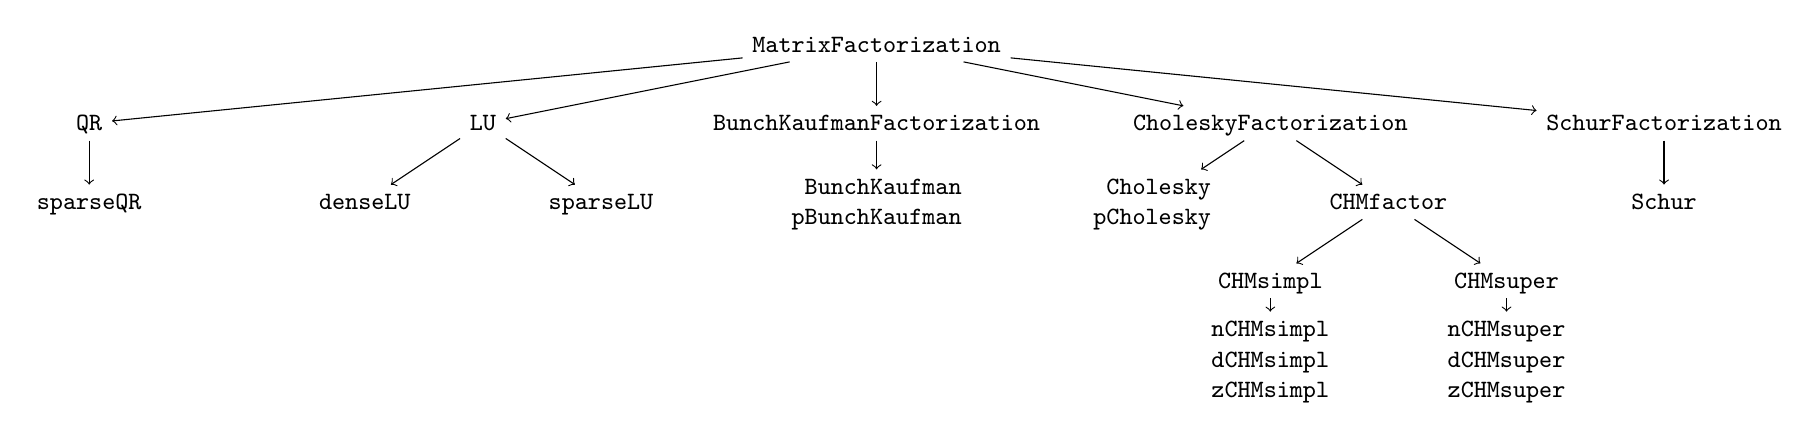
\begin{tikzpicture}[font=\small \tt,text depth=0pt,align=right]
\graph [no placement]
{
        MatrixFactorization[x=  0.0,y= 0],

                         QR[x=-10.0,y=-1],
                         LU[x=- 5.0,y=-1],
  BunchKaufmanFactorization[x=  0.0,y=-1],
      CholeskyFactorization[x=  5.0,y=-1],
         SchurFactorization[x= 10.0,y=-1],

                   sparseQR[x=-10.0,y=-2],
                    denseLU[x=- 6.5,y=-2],
                   sparseLU[x=- 3.5,y=-2],
               BunchKaufman[x=  0.0,y=-2,as={BunchKaufman \\ pBunchKaufman}],
                   Cholesky[x=  3.5,y=-2,as={Cholesky     \\ pCholesky    }],
                  CHMfactor[x=  6.5,y=-2],
                      Schur[x= 10.0,y=-2],

                   CHMsimpl[x=  5.0,y=-3],
                   CHMsuper[x=  8.0,y=-3],

                        Lsi[x=  5.0,y=-4,as={nCHMsimpl \\ dCHMsimpl \\ zCHMsimpl}],
                        Lsu[x=  8.0,y=-4,as={nCHMsuper \\ dCHMsuper \\ zCHMsuper}],

  MatrixFactorization -> { QR, LU, BunchKaufmanFactorization, CholeskyFactorization, SchurFactorization },
  QR -> sparseQR,
  LU -> { denseLU, sparseLU },
  BunchKaufmanFactorization -> BunchKaufman,
  CholeskyFactorization -> { Cholesky, CHMfactor -> { CHMsimpl -> Lsi, CHMsuper -> Lsu } },
  SchurFactorization -> Schur
};
\end{tikzpicture}
\end{document}
